\documentclass{beamer}

\mode<presentation>						% Set options
{
  \usetheme{Hannover}					% Set theme
  \usecolortheme{rose} 				% Set colors
  % \usefonttheme{structurebold}  				% Set font theme
  \setbeamertemplate{caption}[numbered]	% Set caption to be numbered
}

% % Uncomment this to have the outline at the beginning of each section highlighted.
% \AtBeginSection[]
% {
%   \begin{frame}
%     \tableofcontents[currentsection]
%   \end{frame}
% }

\usepackage[varg]{txfonts}
\usepackage[T1]{fontenc}
\usepackage[sfdefault,scaled=0.95]{FiraSans}
\usepackage[small,euler-digits]{eulervm}
\usepackage{inconsolata}
\usepackage{textcomp}
\usepackage{graphicx}					% For including figures
\usepackage{booktabs}					% For table rules
\usepackage{hyperref}					% For cross-referencing

\title[Towards Categorical Metadata]{Towards Categorical Metadata\\ for Unreduced Climate Observations}
\author[C.~Grainger]{Colton Grainger}
\institute{University of Colorado Boulder}
\date{\today}

\usepackage[all]{xy}
\usepackage{listings}

\begin{document}

% front
\begin{frame}
    \hspace{-5.65em}
\includegraphics[width=4.28em]{img/slides_qrcode.png}$\xymatrix{& \mathsf{slides} \ar[l]}$
\titlepage
\begin{figure}
    
\includegraphics[height=4.5em]{img/CISL-contemp-logo-blue-square}\hspace{0.5em}
    
\includegraphics[height=5em]{img/cu-logo}\hspace{0.5em}
    
\includegraphics[height=5em]{img/nsf-logo}
\end{figure}
\end{frame}

% "tasks"
\section{Status Quo}

\begin{frame}

    \begin{center}
        unreduced data from $\sim$100 Tb collection of images (ACRE)
    \end{center}


    \begin{beamerboxesrounded}{marine logbooks 1870--1950}
        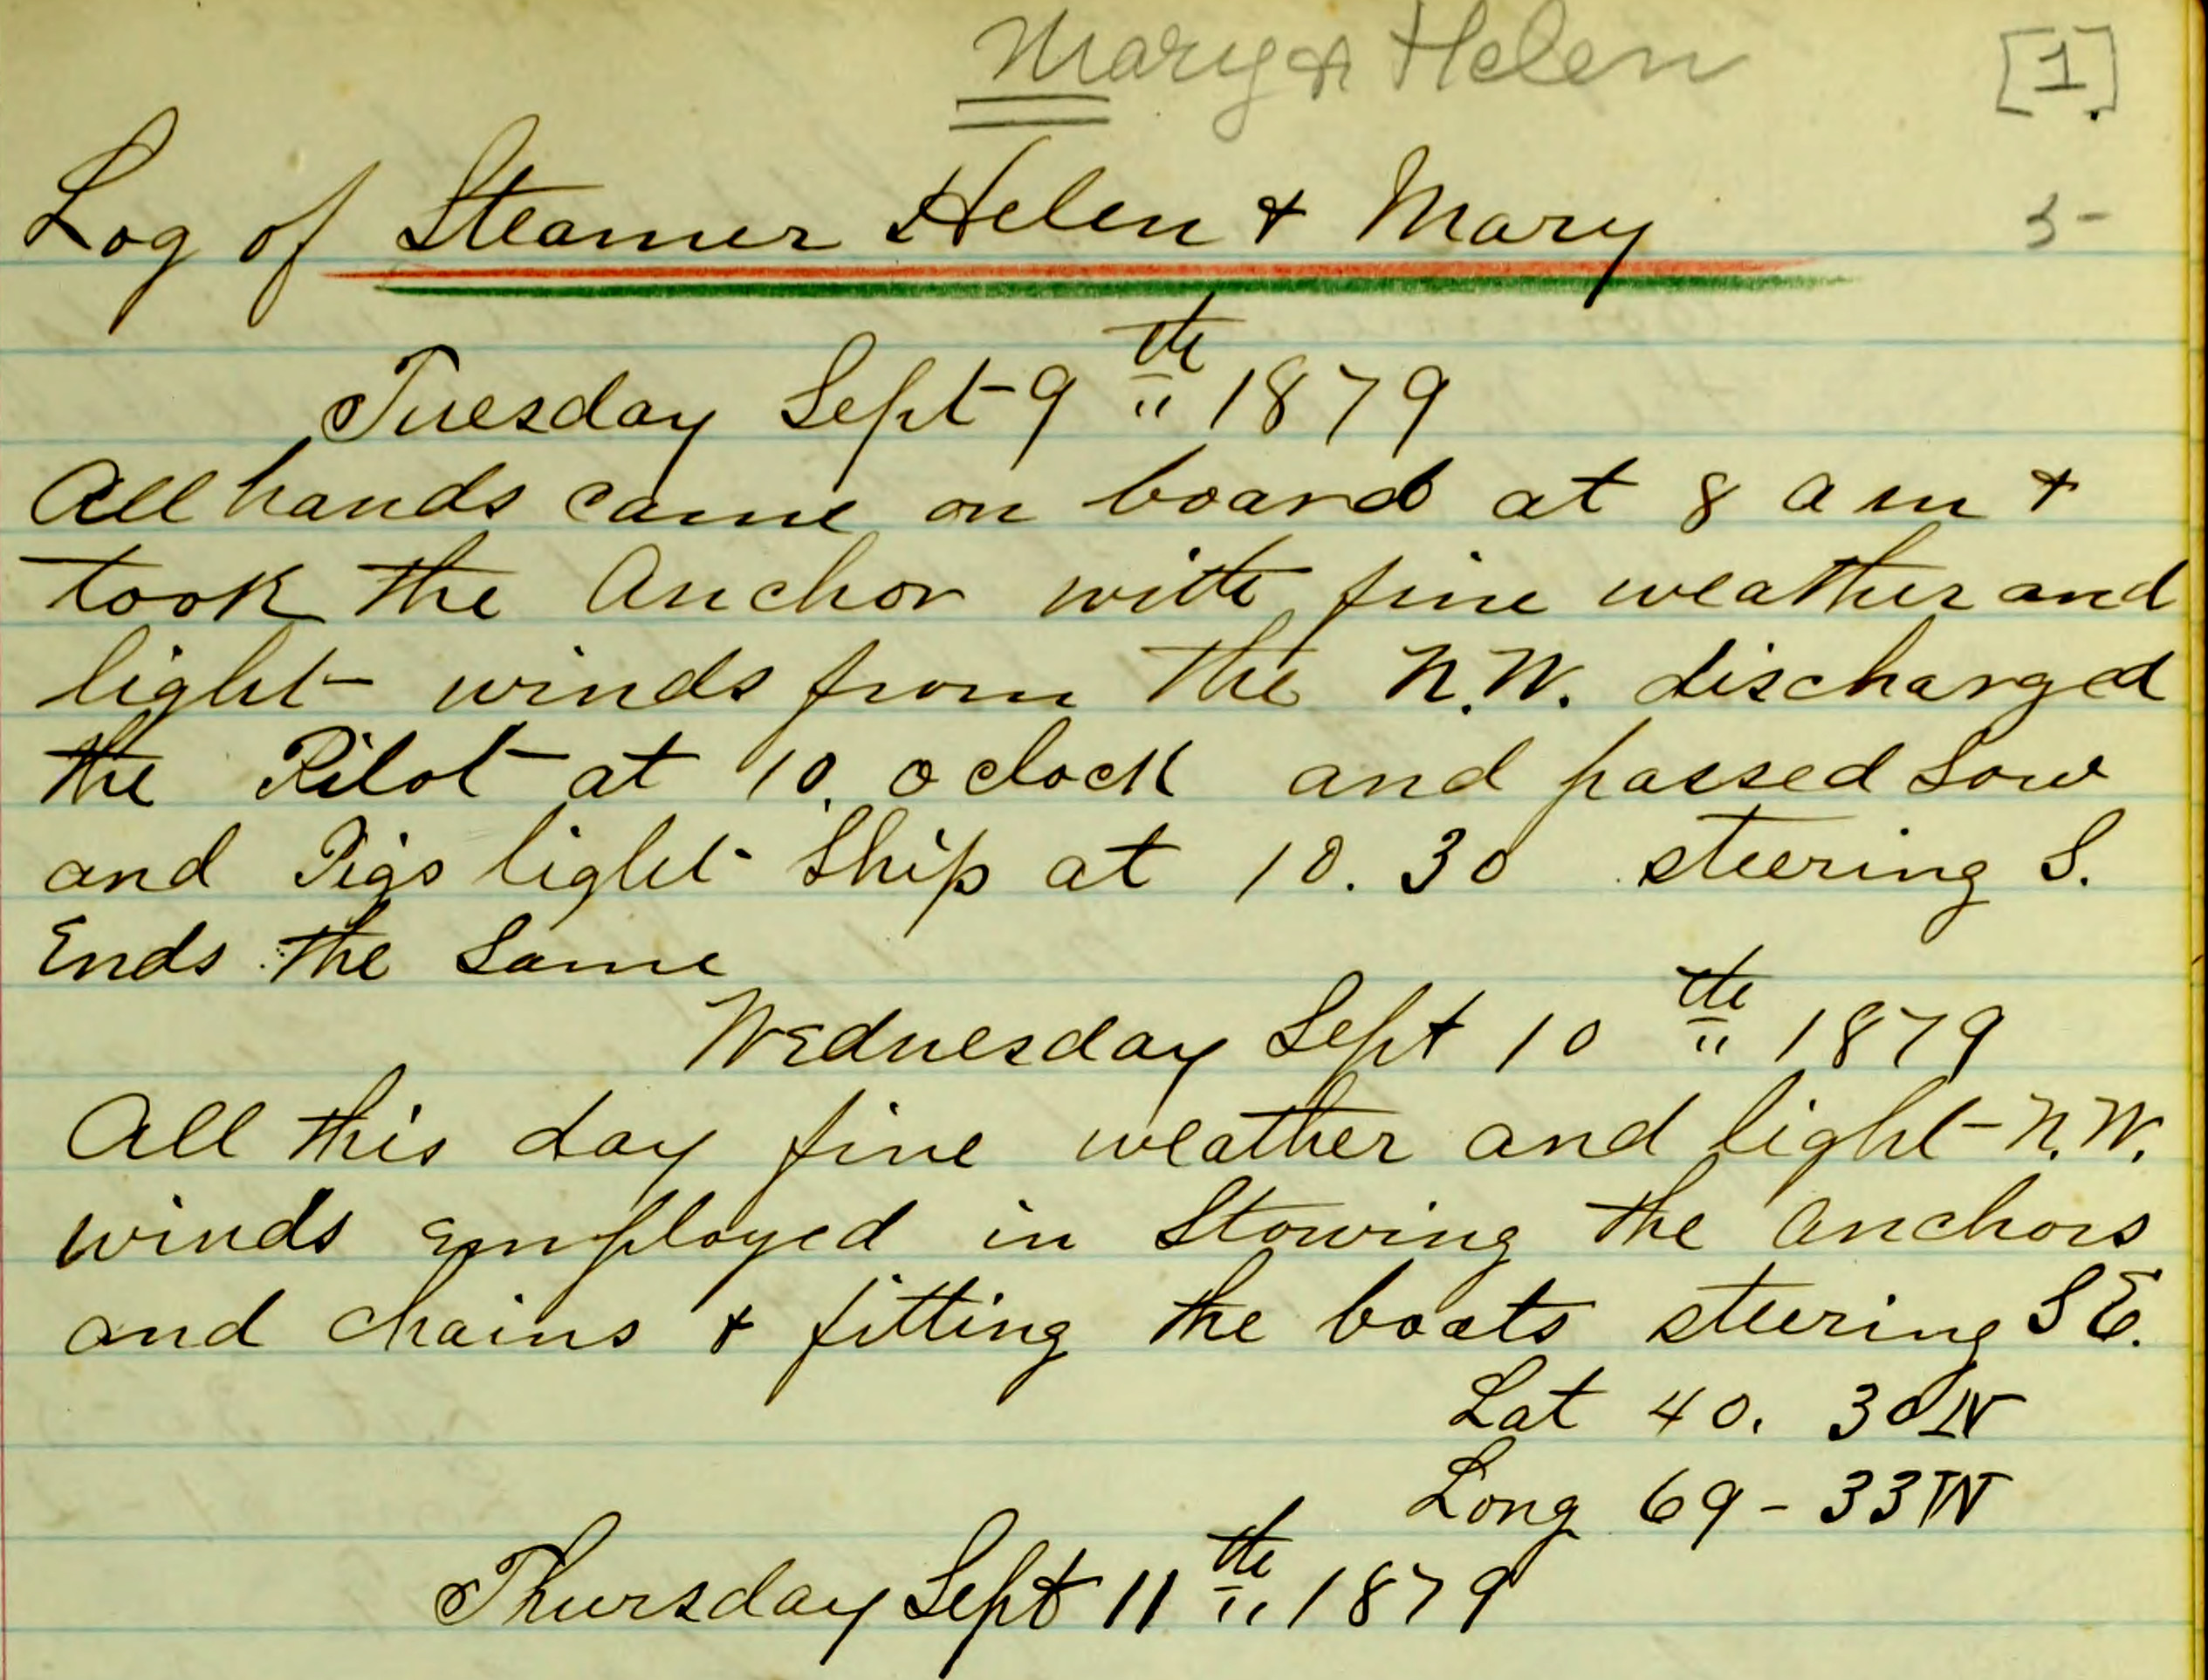
\includegraphics[height=12.5em]{img/mary-1879}
        \hspace{0.5em}
        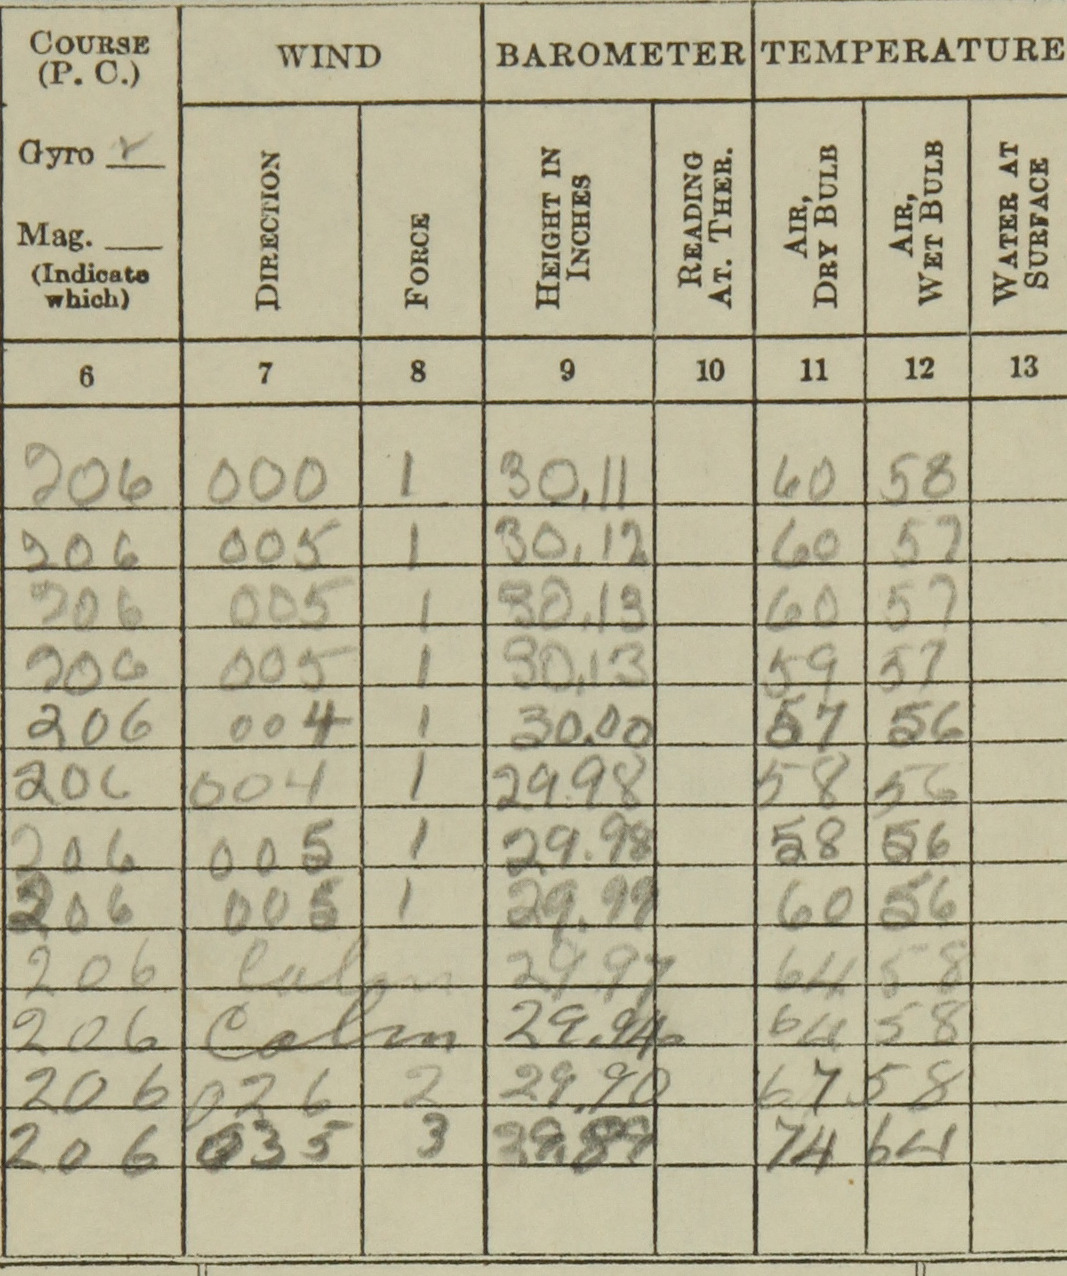
\includegraphics[height=12.5em]{img/idaho-1944}
    \end{beamerboxesrounded}
    \vfill

    \begin{beamerboxesrounded}{land stations 1870--1930}
        Indian Daily Weather Reports, Todd Folios, etc.
    \end{beamerboxesrounded}

\end{frame}

\begin{frame}[fragile]
    \begin{example}[reduction of 6Mb image to a 2Kb time series]
        \begin{figure}
            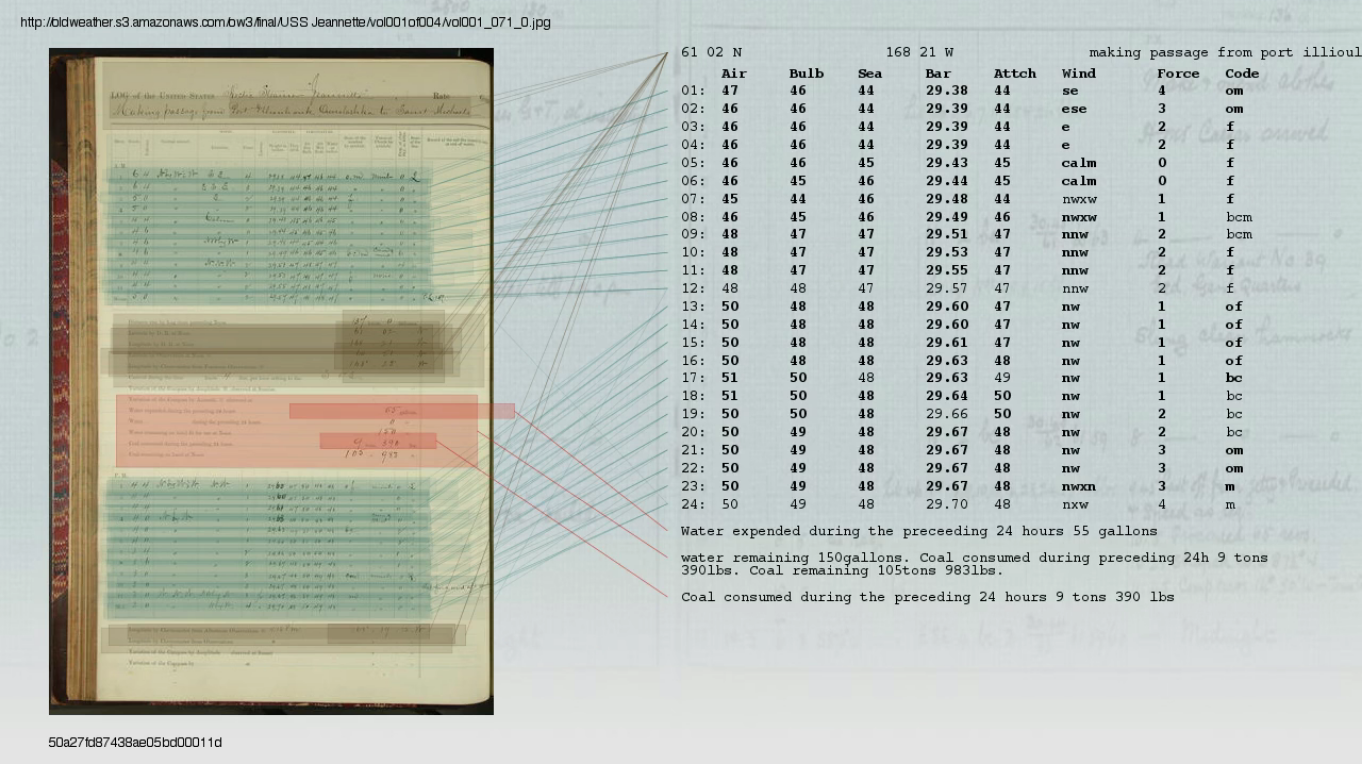
\includegraphics[width=\textwidth]{img/2019-07-30-jeannette}
            \caption{
                24 hours on the USS Jeannette (P. Brohan)
            }
        \end{figure}
    \end{example}
\end{frame}

\begin{frame}[fragile]
  \begin{beamerboxesrounded}{\textit{url}}
        \url{twitter.com/NCAR\_RDA/status/1144058111654711296}
  \end{beamerboxesrounded}

  \begin{minipage}[t]{0.43\linewidth}
      \begin{figure}
      \textit{qrcode}
          
\includegraphics[width=\textwidth]{img/brohan_qrcode}
          \caption{
            \emph{CISL Seminar}, P. Brohan (2019)
          }
      \end{figure}
  \end{minipage}
  \begin{minipage}[t]{0.55\linewidth}
      \begin{example}
      \begin{itemize}
        \item $2^6$ bytes $\sim$ 70 ASCII characters
        \item $2^{12}$ bytes $\sim$ $441 \times 441$ pixels
        \item a \texttt{qrcode} \textbf{reduces} to a \texttt{url}
      \end{itemize}
    \end{example}

\begin{verbatim}
$ exiftool brohan_qrcode.png
File Size : 2.7 kB
Image Size : 441x441
\end{verbatim}
\end{minipage}
\end{frame}

\begin{frame}[fragile]
  \begin{center}
    \textit{metadata}\\
    \texttt{\{'key:value' for key in <schema>\}}
  \end{center}

    \textit{what metadata is signal? or only noise?}

\begin{minipage}[t]{0.5\linewidth}
    \begin{figure}
        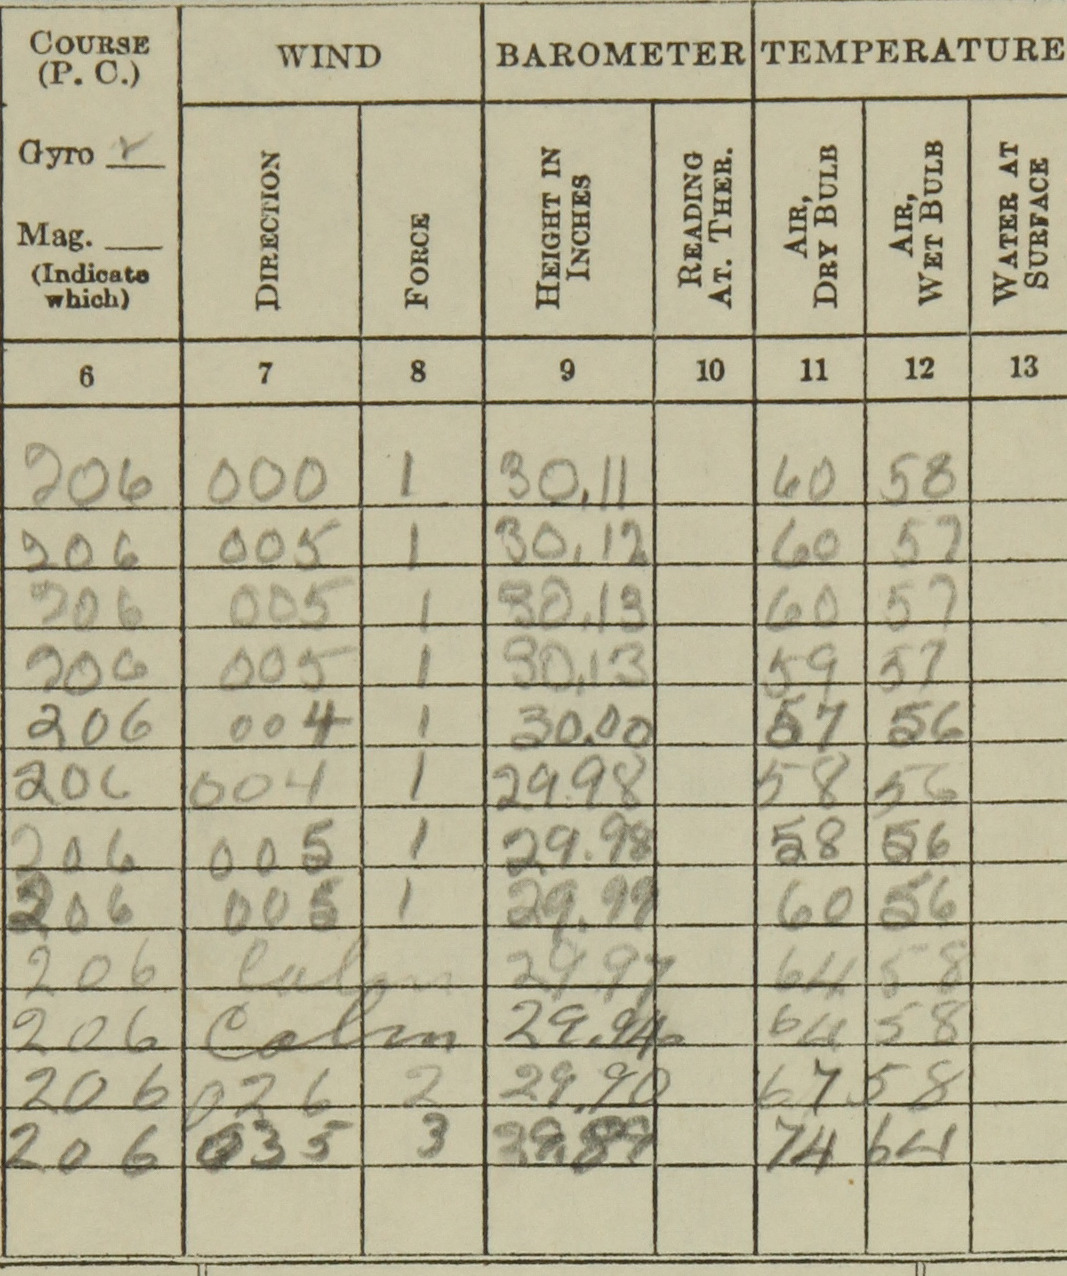
\includegraphics[width=0.9\textwidth]{img/idaho-1944}
        \caption{
            May 1944, Idaho (BB-42)
        }
    \end{figure}
\end{minipage}
%either math model or schema here TODO
\begin{minipage}[t]{0.45\linewidth}
    \begin{figure}
        \begin{itemize}
            \item archive
            \item document
            \item image
            \item observation
            \item platform
        \end{itemize}
        \caption{metadata classes}
    \end{figure}
\end{minipage}
\end{frame}

\section{Proposal}
\begin{frame}
    \begin{enumerate}
        \item Gather images at a \textbf{single resource}.
        \item Establish a \textbf{common description framework} for image metadata.
        \item Provide \textbf{bulk, programmatic access} to image subsets.
    \end{enumerate}
\end{frame}

\section{Functions}

\begin{frame}
    \begin{enumerate}
        \item MySQL schema with Makefile.
        \item Agnostic ingest scripts. \texttt{assign\_uuid()}. Bundle metadata.
        \item \texttt{rda.ucar.edu/i/<uuid>}
    \end{enumerate}
\end{frame}

\section{Interfaces}
\begin{frame}
	\begin{enumerate}
        \item RELAX NG validator.

        \item Python pandas interface. Query methods.

        \item \texttt{rda.ucar.edu/i/<query>}
	\end{enumerate}
\end{frame}

\section{References}
\begin{frame}
    \begin{figure}
        
\includegraphics[width=\0.9\textwidth]{img/git_qr.png}
        \caption{git repo}
    \end{figure}
\end{frame}
\end{document}
